\documentclass{article}
\usepackage{graphicx}
\usepackage[utf8]{inputenc}

\setlength\fboxsep{0pt}
\setlength\fboxrule{0.5pt}

\title{
    Requirements and Analysis Document for group 16
    \author{Erik Sjöström,
            Filip Labe,
            Jonatan Källman,
            Sarosh J. Nasir}
    \date{\today \\v1.0}         
}

\begin{document}
\maketitle

\section{Introduction}
We have indentified a huge gap in the world of clicker games, namely 
Lord of the Rings based clicker games. Our project aims to fill that gap. \\
This game will simulate the adventure of Frodo and friends on their quest to
destroy the one ring, and will benifit anyone who likes both LOTR and clickers.\\
This game might be useful on the bus, to pass the time when moving between locataions, or when sitting on the toilet. 

\subsection{Definitions, acronyms, abbriviations}
LOTR: Lord of the Rings.

\section{Requirements}
\subsection{User interface}
\subsection{Functional requirements}
\begin{itemize}
    \item Attack
    \item Open map
    \item Use map
    \item Buy upgrades
    \item Go home
    \item Improve home
    \item Check stats
\end{itemize}
\subsection{Non-functional requirements}

\section{Use cases}
\subsection{Usability model}
\fbox{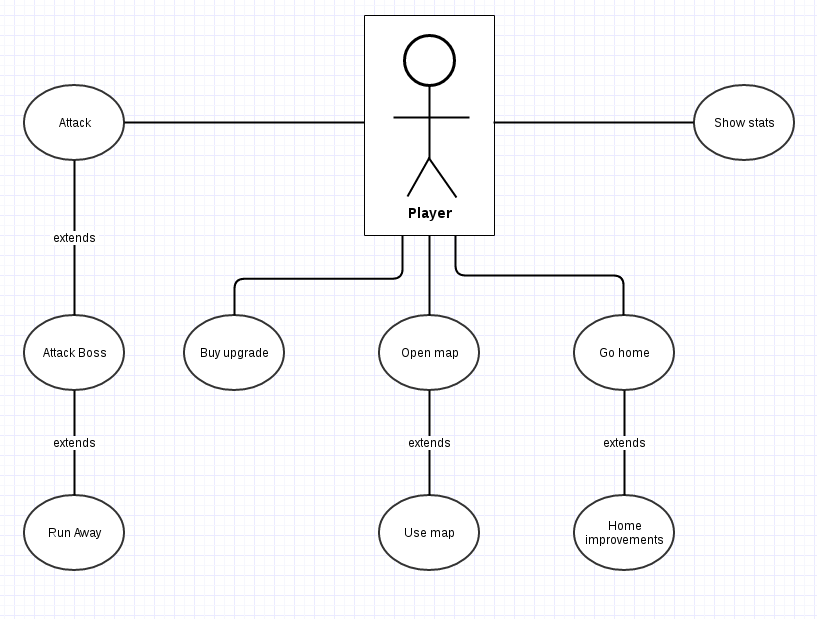
\includegraphics[scale=0.4]{usabilityModel.png}}
\subsection{Use case listings}
\subsubsection{Use case: Attack}
Summary: The user clicks the screen and the game calculates new health for the monster.\\
Priority: High\\
Extends: undefined\\
Includes: undefined\\
Participators: Player\\
Normal flow of event: The player attacks the monster and the monster survives.
\begin{tabular}{| c | l | l |} \hline
    & Actor & System \\ \hline
    1 & Player clicks screen & \\ \hline
    2 & & Attack animation plays \\ \hline
    3 & & Calculate new health for monster\\ \hline
\end{tabular}\\
Alternate flow: The player attacks the monster and the monster dies. The level is not cleared.\\
\begin{tabular}{| c | l | l |} \hline
    & Actor & System \\ \hline
    1 & Player clicks screen & \\ \hline
    2 & & Attack animation plays \\ \hline
    3 & & Calculate new health for monster\\ \hline
    4 & & Health $\le$ 0 \\ \hline
    5 & & Death animation plays \\ \hline 
    6 & & Replace dead monster with new monster \\ \hline
    7 & Player gets money & \\ \hline
\end{tabular}\\
Alternate flow: The player attacks the monster and the monster dies. The level is cleared.\\
\begin{tabular}{| c | l | l |} \hline
    & Actor & System \\ \hline
    1 & Player clicks screen & \\ \hline
    2 & & Attack animation plays \\ \hline
    3 & & Calculate new health for monster\\ \hline
    4 & & Health $\le$ 0 \\ \hline
    5 & & Death animation plays \\ \hline 
    6 & & Replace dead monster with new monster \\ \hline
    7 & & The option to change level is made avliable\\ \hline
    8 & The player gets money & \\ \hline
\end{tabular}

\subsubsection{Use case: Attack boss}
Summary: The player is fighting a boss \\
Priority: High \\
Extends: Attack\\
Includes: \\
Participators: Player \\
Normal flow of event: The player attacks the boss and defeats it within the time frame \\
\begin{tabular}{|c|l|l|} \hline
    & Actor & System \\ \hline
    1 & Player clicks screen & \\ \hline
    2 & & Attack animation plays \\ \hline
    3 & & Calculate new health for boss \\ \hline
    4 & & Death animation plays \\ \hline
    5 & & Unlock next level \\ \hline
    6 & & Replace boss \\ \hline
    7 & Player gets money & \\ \hline
\end{tabular}\\
Normal flow of event: The player attacks the boss and does not defeat it, but is still within the time frame \\
\begin{tabular}{|c|l|l|} \hline
    & Actor & System \\ \hline
    1 & Player clicks screen & \\ \hline
    2 & & Attack animation plays \\ \hline
    3 & & Calculate new health for boss \\ \hline
\end{tabular}\\
Alternate event: The player does not defeat the boss within the time frame \\
\begin{tabular}{|c|l|l|} \hline
    & Actor & System \\ \hline
    1 & & Replace boss \\ \hline
\end{tabular}
\subsubsection{Use case: Run away}
Summary: The player wants to run away from the fight.\\
Priority: Medium \\
Extends: Attack boss\\
Includes:\\
Participators: Player\\
Normal flow of the event: The player clicks the "run away" button.\\
\begin{tabular}{|c|l|l|} \hline
    & Actor & System \\ \hline
    1 & The player clicks the button & \\ \hline
    2 & & Sends the player to Home \\ \hline
\end{tabular}

\subsubsection{Use case: Buy upgrade}
Summary: The user tries to buy an upgrade.\\
Priority: Medium\\
Extends: undefined\\
Includes: undefined\\
Participators: Player\\
Normal flow of event: The player clicks on the upgrade and has enough money.\\
\begin{tabular}{|c|l|l|} \hline
      & Actor & System \\ \hline
    1 & Player clicks on the upgrade & \\ \hline
    2 & & Checks that the player has enough money to buy the upgrade \\ \hline
    3 & & The upgrade is applied to the player \\ \hline
\end{tabular}\\ 
Alternate flow: The player clicks on the upgrade but does not have enough money. \\
\begin{tabular}{|c|l|l|} \hline
      & Actor & System \\ \hline
    1 & Player clicks on the upgrade & \\ \hline
    2 & & Checks that the player has enough money to buy the upgrade \\ \hline
\end{tabular} 

\subsubsection{Use case: Open map}
Summary: The player clicks the button labeled "map"
Priority: Medium \\
Extends: undefined\\
Includes: undefined\\
Participators: Player \\
Normal flow of event: The player clicks the button labeled "map"\\
\begin{tabular}{|c|l|l|} \hline
      & Actor & System \\ \hline
    1 & Player clicks on the button & \\ \hline
    2 & & Displays map page \\ \hline
\end{tabular} 

\subsubsection{Use case: Use map}
Summary: The user tries to move to a different level.\\
Priority: High\\
Extends: undefined\\
Includes: undefined\\
Participators: Player \\
Normal flow of event: The player clicks on the level they want to move to, the level is unlocked.\\
\begin{tabular}{|c|l|l|} \hline
      & Actor & System \\ \hline
    1 & Player clicks on the level & \\ \hline
    2 & & Checks that the level is unlocked \\ \hline
    3 & & Loads new level \\ \hline
\end{tabular} \\
Alternate flow of event: The player clicks on the level they want to move to, the level is locked.\\
\begin{tabular}{|c|l|l|} \hline
      & Actor & System \\ \hline
    1 & Player clicks on the level & \\ \hline
    2 & & Checks that the level is unlocked \\ \hline
\end{tabular} 

\subsubsection{Use case: Show stats}
Summary: The use clicks the button labeled "Stats"\\
Priority: low\\
Extends: undefined\\
Includes: undefined\\
Participators: Player\\
Normal flow of event: The player clicks the button labled "Stats"\\
\begin{tabular}{|c|l|l|} \hline
      & Actor & System \\ \hline
    1 & Player clicks on the button & \\ \hline
    2 & & Displays stats page \\ \hline
\end{tabular} 

\subsubsection{Use case: Go home}
Summary: The user wants to go home\\
Priority: Low \\
Extends: undefined\\
Includes: undefined\\
Participators: Player \\
Normal flow of event: The player clicks the button labeled "Home"\\
\begin{tabular}{|c|l|l|} \hline
      & Actor & System \\ \hline
    1 & Player clicks on the button & \\ \hline
    2 & & Displays the player home screen \\ \hline
\end{tabular} 

\subsubsection{Use case: Home improvements}
Summary: The user wants to improve their home\\
Priority: low \\
Extends: undefined\\
Includes: undefined\\
Participators: Player\\
Normal flow of event: The player wants to buy an animal, has enough money and enough space.\\
\begin{tabular}{|c|l|l|} \hline
      & Actor & System \\ \hline
    1 & & Checks that player has enough money \\ \hline
    2 & & Checks that player has enough space \\ \hline
    3 & & Enables button. \\ \hline
    4 & Player clicks on a buy animal button & \\ \hline
    5 & & Deduct money from player \\ \hline
    6 & & Add animal to home \\ \hline
\end{tabular}  \\
Alternate flow: The player wants to buy an animal, does not have enough money 
\begin{tabular}{|c|l|l|} \hline
      & Actor & System \\ \hline
    1 & & Checks that player has enough money \\ \hline
    2 & & Checks that the player has enough space \\ \hline
    3 & & Does not enable button \\ \hline
\end{tabular}  \\
Alternate flow: The player wants to buy an animal, does not have enough space 
\begin{tabular}{|c|l|l|} \hline
      & Actor & System \\ \hline
    1 & & Checks that player has enough money \\ \hline
    2 & & Checks that the player has enough space \\ \hline
    3 & & Does not enable button \\ \hline
\end{tabular}  \\
Alternate flow: The player wants to buy more space, has enough money.\\
\begin{tabular}{|c|l|l|} \hline
    & Actor & System \\ \hline
    1 & & Check that the player has enough money \\ \hline
    2 & & Enables button. \\ \hline
    3 & Player clicks on button \\ \hline
    4 & & Deduct money from player \\ \hline
    5 & & Add more space to player \\ \hline
\end{tabular}\\
Alternate flow: The player wants to buy more space, does not have enough money.\\
\begin{tabular}{|c|l|l|} \hline
    & Actor & System \\ \hline
    1 & & Check that the player has enough money \\ \hline
    2 & & Does not enable button. \\ \hline
\end{tabular}\\
Alternate flow: The player wants to sell an animal, has animals.\\
\begin{tabular}{|c|l|l|} \hline
    & Actor & System \\ \hline
    1 & & Checks that player has animals \\ \hline
    2 & & Enable button \\ \hline
    3 & Player clicks button & \\ \hline
    4 & & Remove one animal from player \\ \hline
    5 & & Add money to player \\ \hline
\end{tabular}\\
Alternate flow: The player wants to sell an animal, has no animals.\\
\begin{tabular}{|c|l|l|} \hline
    & Actor & System \\ \hline
    1 & & Checks that player has animals \\ \hline
    2 & & Does not enable button \\ \hline
\end{tabular}

\section{Domain model}
\fbox{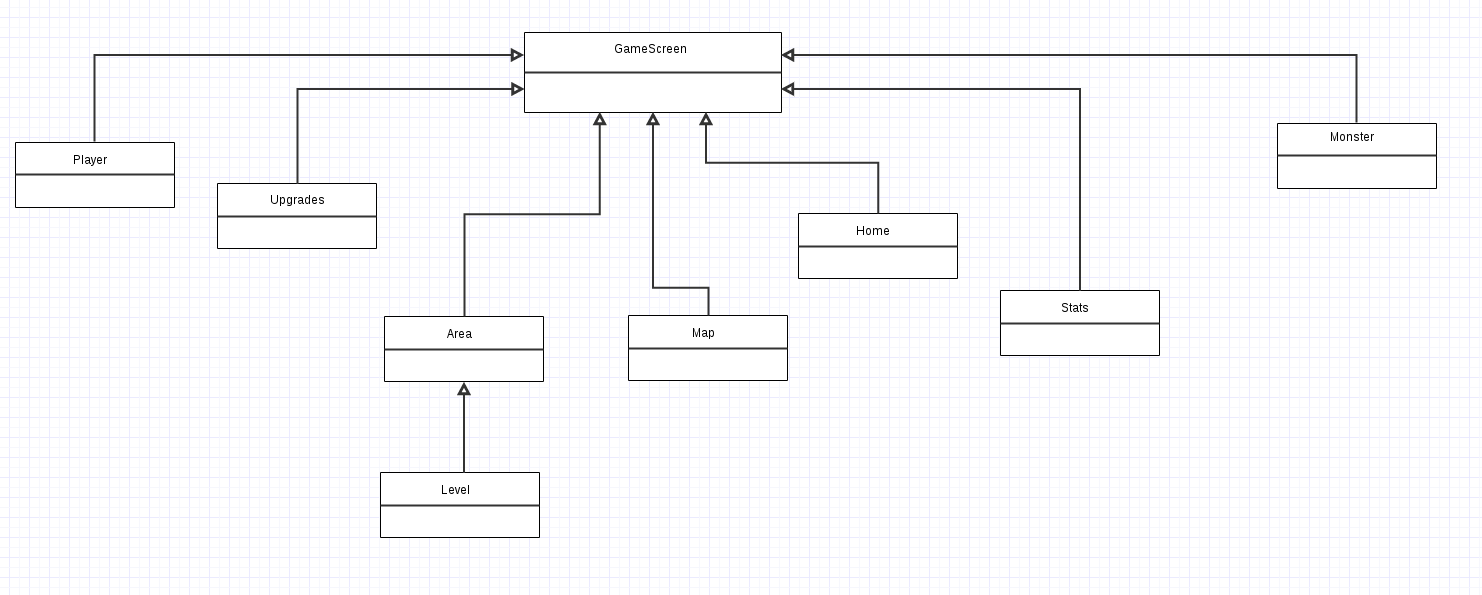
\includegraphics[scale=0.3]{domainModel.png}}

\subsection{Class responsibilities}
\subsubsection{Game screen}
Combines all other classes into one unified interface.
\subsubsection{Player}
The actual player. Has money, animals, space, and an amount of damage.
\subsubsection{Monster}
A bad guy. Has health points, and an amount of money to drop.
\subsubsection{Stats}
A view for the players stats.
\subsubsection{Map}
A view for a map over the levels that a player can travel to.
\subsubsection{Upgrades}
A view over the upgrades that a player can buy.
\subsubsection{Home}
The players home. Here the player can buy animals which earn passive money. 
\subsubsection{Area}
An area, has a name, and a list of levels associated with that area.
\subsubsection{Level}
Determines how hard the monsters are, and how much money they drop.
\section{References}
\end{document}

